\chapter{Návrh}
\label{ch:navrh}

Od vyvíjené aplikace je vyžadována vysoká spolehlivost. Proto musí být pečlivě otestováná přímo v prostředí FN Plzeň na nemocniční databázi a proveden testovací provoz. Na oddělení bude více tabletů pro případ, že by se některý rozbil či ztratil. Při selhání aplikace mohou sestry vždy použít program WinMedicalc nainstalovaný na počítači v sesterně, který je přímo připojen do interní sítě nemocnice. Výpadek databázového serveru nebo sítě řeší SIS FN Plzeň.

\section{Architektura}

Aplikace je rozdělena do tří vrstev (viz obrázek \ref{fig:architektura}). Vrstva přístupu k databázi se stará o spojení s databází, stahování a odesílání dat. Logická vrstva se stará o zpracování dat z databáze do formy, která je zobrazitelná v uživatelském rozhraní, a poskytuje uživatelskému rozhraní prostředky pro práci s~daty. Také ošetřuje zadávání nekorektních dat. Vrstva uživatelského rozhraní se stará o zobrazení dat uživateli a umožňuje mu manipulaci s daty.

\begin{figure}[H]
	\centering
	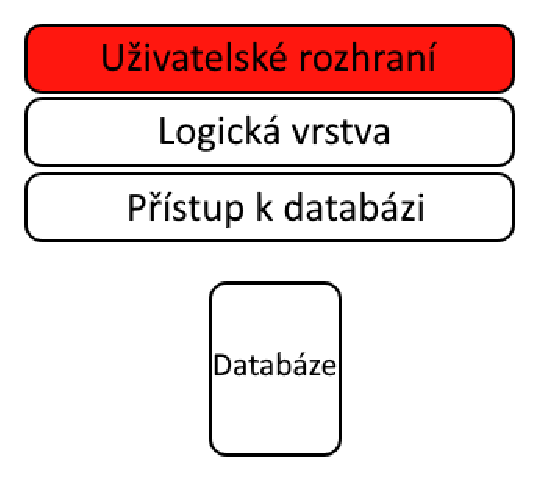
\includegraphics[width=0.5\textwidth]{img/architektura.eps}
	\caption{Architektura aplikace MediTab}
  \label{fig:architektura}
\end{figure}

Předmětem této práce je vytvoření vrstvy uživatelského rozhraní.


\section{Design}

Uživatelské rozhraní zjednodušuje skutečné procesy v počítači a zprostředkovává komunikaci mezi člověkem a strojem \cite{helander}. Design aplikace musí splňovat požadovanou funkčnost. Zároveň musí být rychlý bez zbytečného klikání, které by zpomalovalo práci.

Ovládání musí být jednoduché. Funkce by měly být zobrazeny pouze, pokud jsou skutečně potřeba, příliš mnoho funkcí rozptyluje uživatele. Základní funkce by měly být zřejmé na první pohled, méně důležité funkce by měly být v pozadí \cite{saffer}. 

Uživatelské rozhraní by mělo být rozděleno na části, které spolu souvisí. Jednotlivé komponenty by měly mít maximálně výstižné názvy.

Typické chyby návrhu uživatelského rozhraní jsou neutříděný obsah oken a menu, nepatřičný vzhled a nadbytečné grafické prvky \cite{sojka}.

Dále by uživatelské rozhraní mělo být intuitivní, podobné technikám, které již uživatel zná, aby nebylo nutné dlouhé zaškolení zdravotních sester. Proto je vhodné přizpůsobit vzhled aplikace co nejvíce vzhledu WinMedicalcu, na který jsou pracovníci FN Plzeň zvyklí, a dodržovat již zavedené konvence. Z toho důvodu jsem zvolil pro grafické uživatelské rozhraní knihovnu WinForms\footnote{System.Windows.Forms} místo novějšího WPF\footnote{Windows Presentation Foundation}.


\section{Uživatelské rozhraní}

Aplikace je určena pro tablet, kdy má vyplňovat celou plochu obrazovky s~minimem prázdného prostoru. Komponenty by měly mít větší velikost pro snazší ovládání na tabletu.

\subsection{Přihlášení}

Jednoduchý dialog pro přihlášení uživatele do aplikace. Obsahuje textové pole pro jméno a pro heslo a dvě tlačítka pro potvrzení a zrušení přihlášení. Automaticky se zobrazí přes hlavní obrazovku při spuštění aplikace.

\subsection{Výběr pacienta}

Po přihlášení se zobrazí seznam pacientů na daném oddělení nebo lůžku (dle výběru z databáze). U každého pacienta bude zobrazeno jeho příjmení, jméno a identifikační číslo (většinou rodné číslo).

V horní části obrazovky bude menu s možností odhlášení uživatele a zobrazení nápovědy. V dolní části statusbar s informacemi o přihlášeném uživateli a verzí aplikace. Vpravo bude tlačítko pro ukončení aplikace.

\subsection{Detail pacienta}

Po výběru pacienta se zobrazí obrazovka s jednotlivými záložkami. Záložky jsou Medikace, Denní bilance tekutin, Hodinová bilance tekutin, Invazivní přístupy a Fyziologie. K dispozici bude vždy jen jedna varianta bilance tekutin dle oddělení, na kterém se tablet nachází (bude určeno v nastavení aplikace).

V dolní části obrazovky bude statusbar s informacemi o přihlášeném uživateli, vybraném pacientovi a s verzí aplikace. Vpravo pak tlačítko pro návrat k výběru pacientů a tlačítko oprav.

\subsubsection{Ordinované léky}

Záložka ordinovaných léků bude podobná tištěné medikační kartě. Jedná se o tabulku s názvem léku, předepsaným dávkováním a jednotlivými hodinami dávkování. V tabulce bude vyznačeno předepsané podání léku šedě a provedené podání léku zeleně s množstvím pro danou hodinu.

\subsubsection{Denní bilance tekutin}

Denní bilance tekutin bude rozdělena na dvě části pro příjem a výdej tekutin stejně, jako tomu je ve WinMedicalcu. Příjem tekutin bude podbarven zeleně, bude obsahovat 7 položek, celkový součet a~tlačítko pro uložení dat. Výdej tekutin bude podbarven červeně, bude obsahovat 5 položek, celkový součet a tlačítko pro uložení dat. U každé položky bude textové pole pro zadání nové celkové hodnoty a textové pole pro zadání nové hodnoty, která se přičte k~původní.

\subsubsection{Hodinová bilance tekutin}

Hodinová bilance bude rozložením podobná denní bilanci tekutin. Pouze místo dvou textových polí bude mít jen jedno pro zadání hodnoty v aktuální hodinu. Dále bude u každé tekutiny tlačítko pro zobrazení seznamu příjmu nebo výdeje tekutiny v jednotlivých hodinách. Do tohoto seznamu se bude moci zapisovat pouze v určitých hodinách dle oddělení.

Tato karta není ve WinMedicalcu.

\subsubsection{Invazivní přístupy}

Záložka invazivních přístupů bude mít podobný vzhled jako ve WinMedicalcu. Každý invazivní přístup bude obsahovat číslo, název, umístění, hloubku zavedení, datum zavedení, počet dnů zavedení, specifikaci, materiál katetru či drénu, stav místa zavedení a tři tlačítka - požadavek na výměnu, výměna a zrušení invazivního přístupu.

Jako poslední položka bude možnost přidání nového invazivního přístupu. Název, umístění a meteriál přístupu se bude vybírat ze seznamu. Datum bude nastaven na aktuální datum a počet dnů na 1. Číslo a hloubka zavedení bude pole s číselnou hodnotou, specifikace a stav bude pole s textovou hodnotou. Tato položka bude mít pouze jedno tlačítko pro přidání.

\subsubsection{Fyziologie}

Záložka fyziologie zobrazuje změřené životní funkce pacieta, tj. teplota, tep, STK\footnote{systoliský tlak krve}, DTK\footnote{diastoliský tlak krve}, frekvence dechu, a také výšku, hmotnost a vypočítané BMI\footnote{body mass index}. Jednotlivé položky bude možné upravovat (kromě BMI, které je spočteno automaticky), smazat, nebo přidat nový zázanam.

\subsection{Opravy}

Po stisknutí tlačítka oprav se zobrazí seznam možných oprav provedených úkonů (ty budou časově omezeny dle oddělení). Každá položka bude obsahovat číslo opravy, datum a čas provedení úkonu, informace o provedeném úkonu a tlačítko pro vrácení úkonu. V dolní části bude tlačítko pro zavření seznamu.